\section{Level description}

The city is loosely based on Venice.

\begin{center}
  \begin{figure}[H]
    \centering
    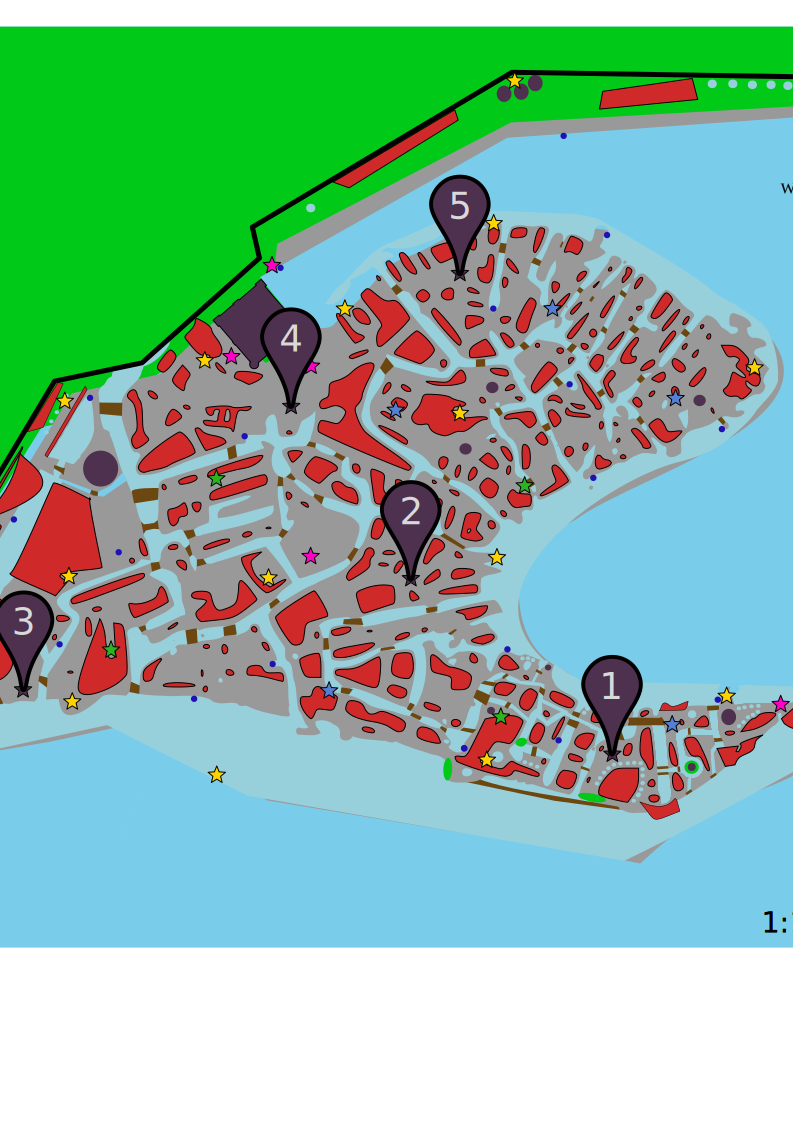
\includegraphics[width=\textwidth]{Images/Maps/dynamia}
    \caption{Map of Dynamia}
  \end{figure}
\end{center}

\newpage

\subsection{Dead end}
\begin{figure}[H]
  \centering
  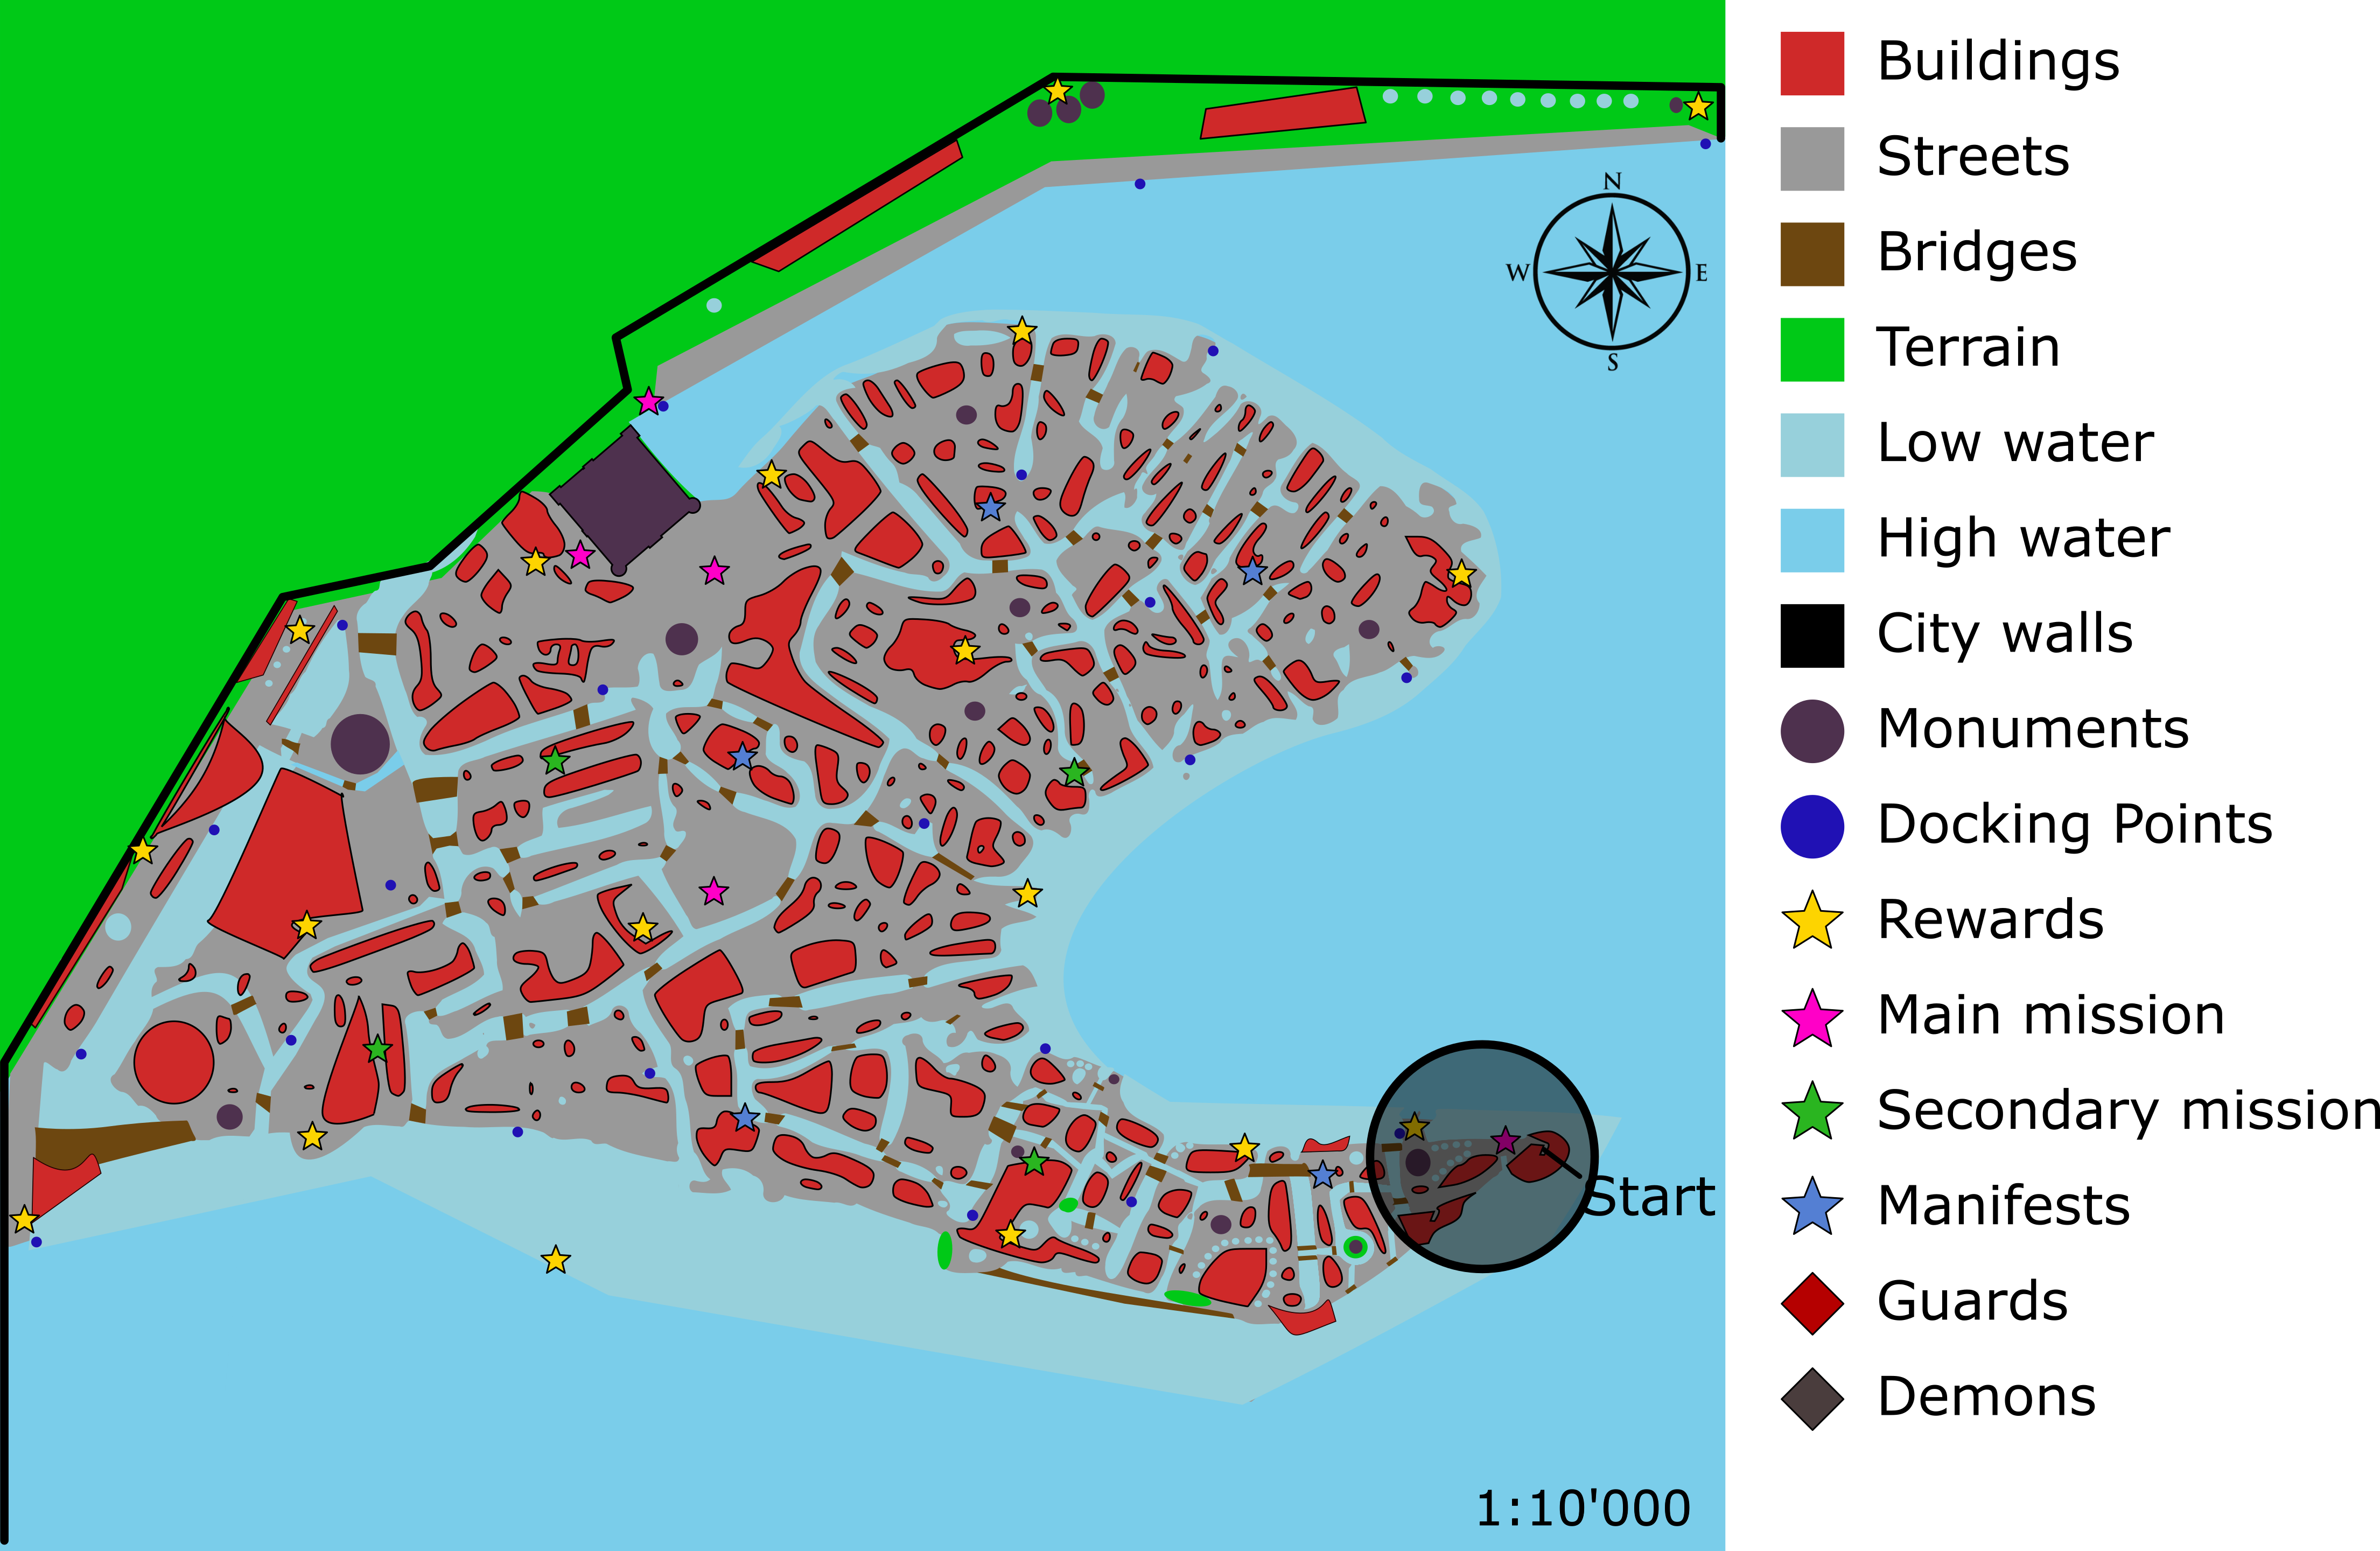
\includegraphics[width=12cm]{Images/Maps/dynamia_deadEnd}
  \caption{Dead end position}
\end{figure}
Dynamia ends here, in a neighbourhood of colored houses that overlook on the canals. Some houses have sea view, instead, the others have their windows on a little, narrow, nice dead-end.
This short street connects the neighbourhood to a big street leading to the central neighbourhoods of Dynamia. \\
At the beginning of this boulevard there is a manifest and a panel with the map of the city. 
The street is bordered by flowerbeds and fountains of every shape and it is loosely based on the \textit{Champs Elysees}.
From every point of the street you can see a big arc of triumph at the end of it that can be considered the entrance of Dynamia
\begin{figure}[H]
    \centering
    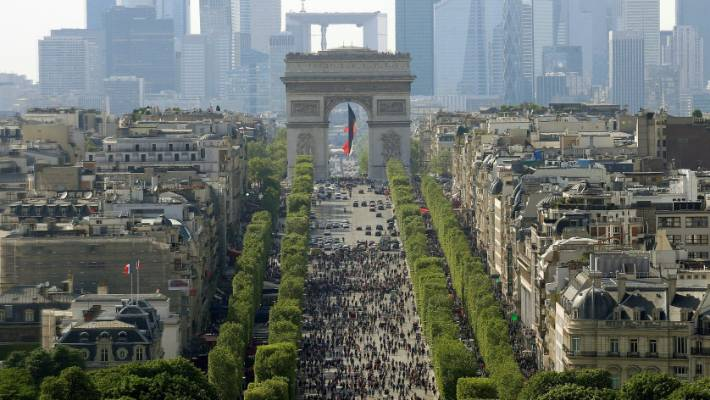
\includegraphics[width=8cm]{Images/Landmarks/arcOfTriumph}
    \caption{A references images of the arc of triumph}
    For more reference images: \href{http://wastelandsteam.altervista.org/dynamia-dead-end}{http://wastelandsteam.altervista.org/dynamia-dead-end}\\Password: \textit{gld18}
  \end{figure}

\subsection{Market of Dynamia}
\begin{figure}[H]
  \centering
  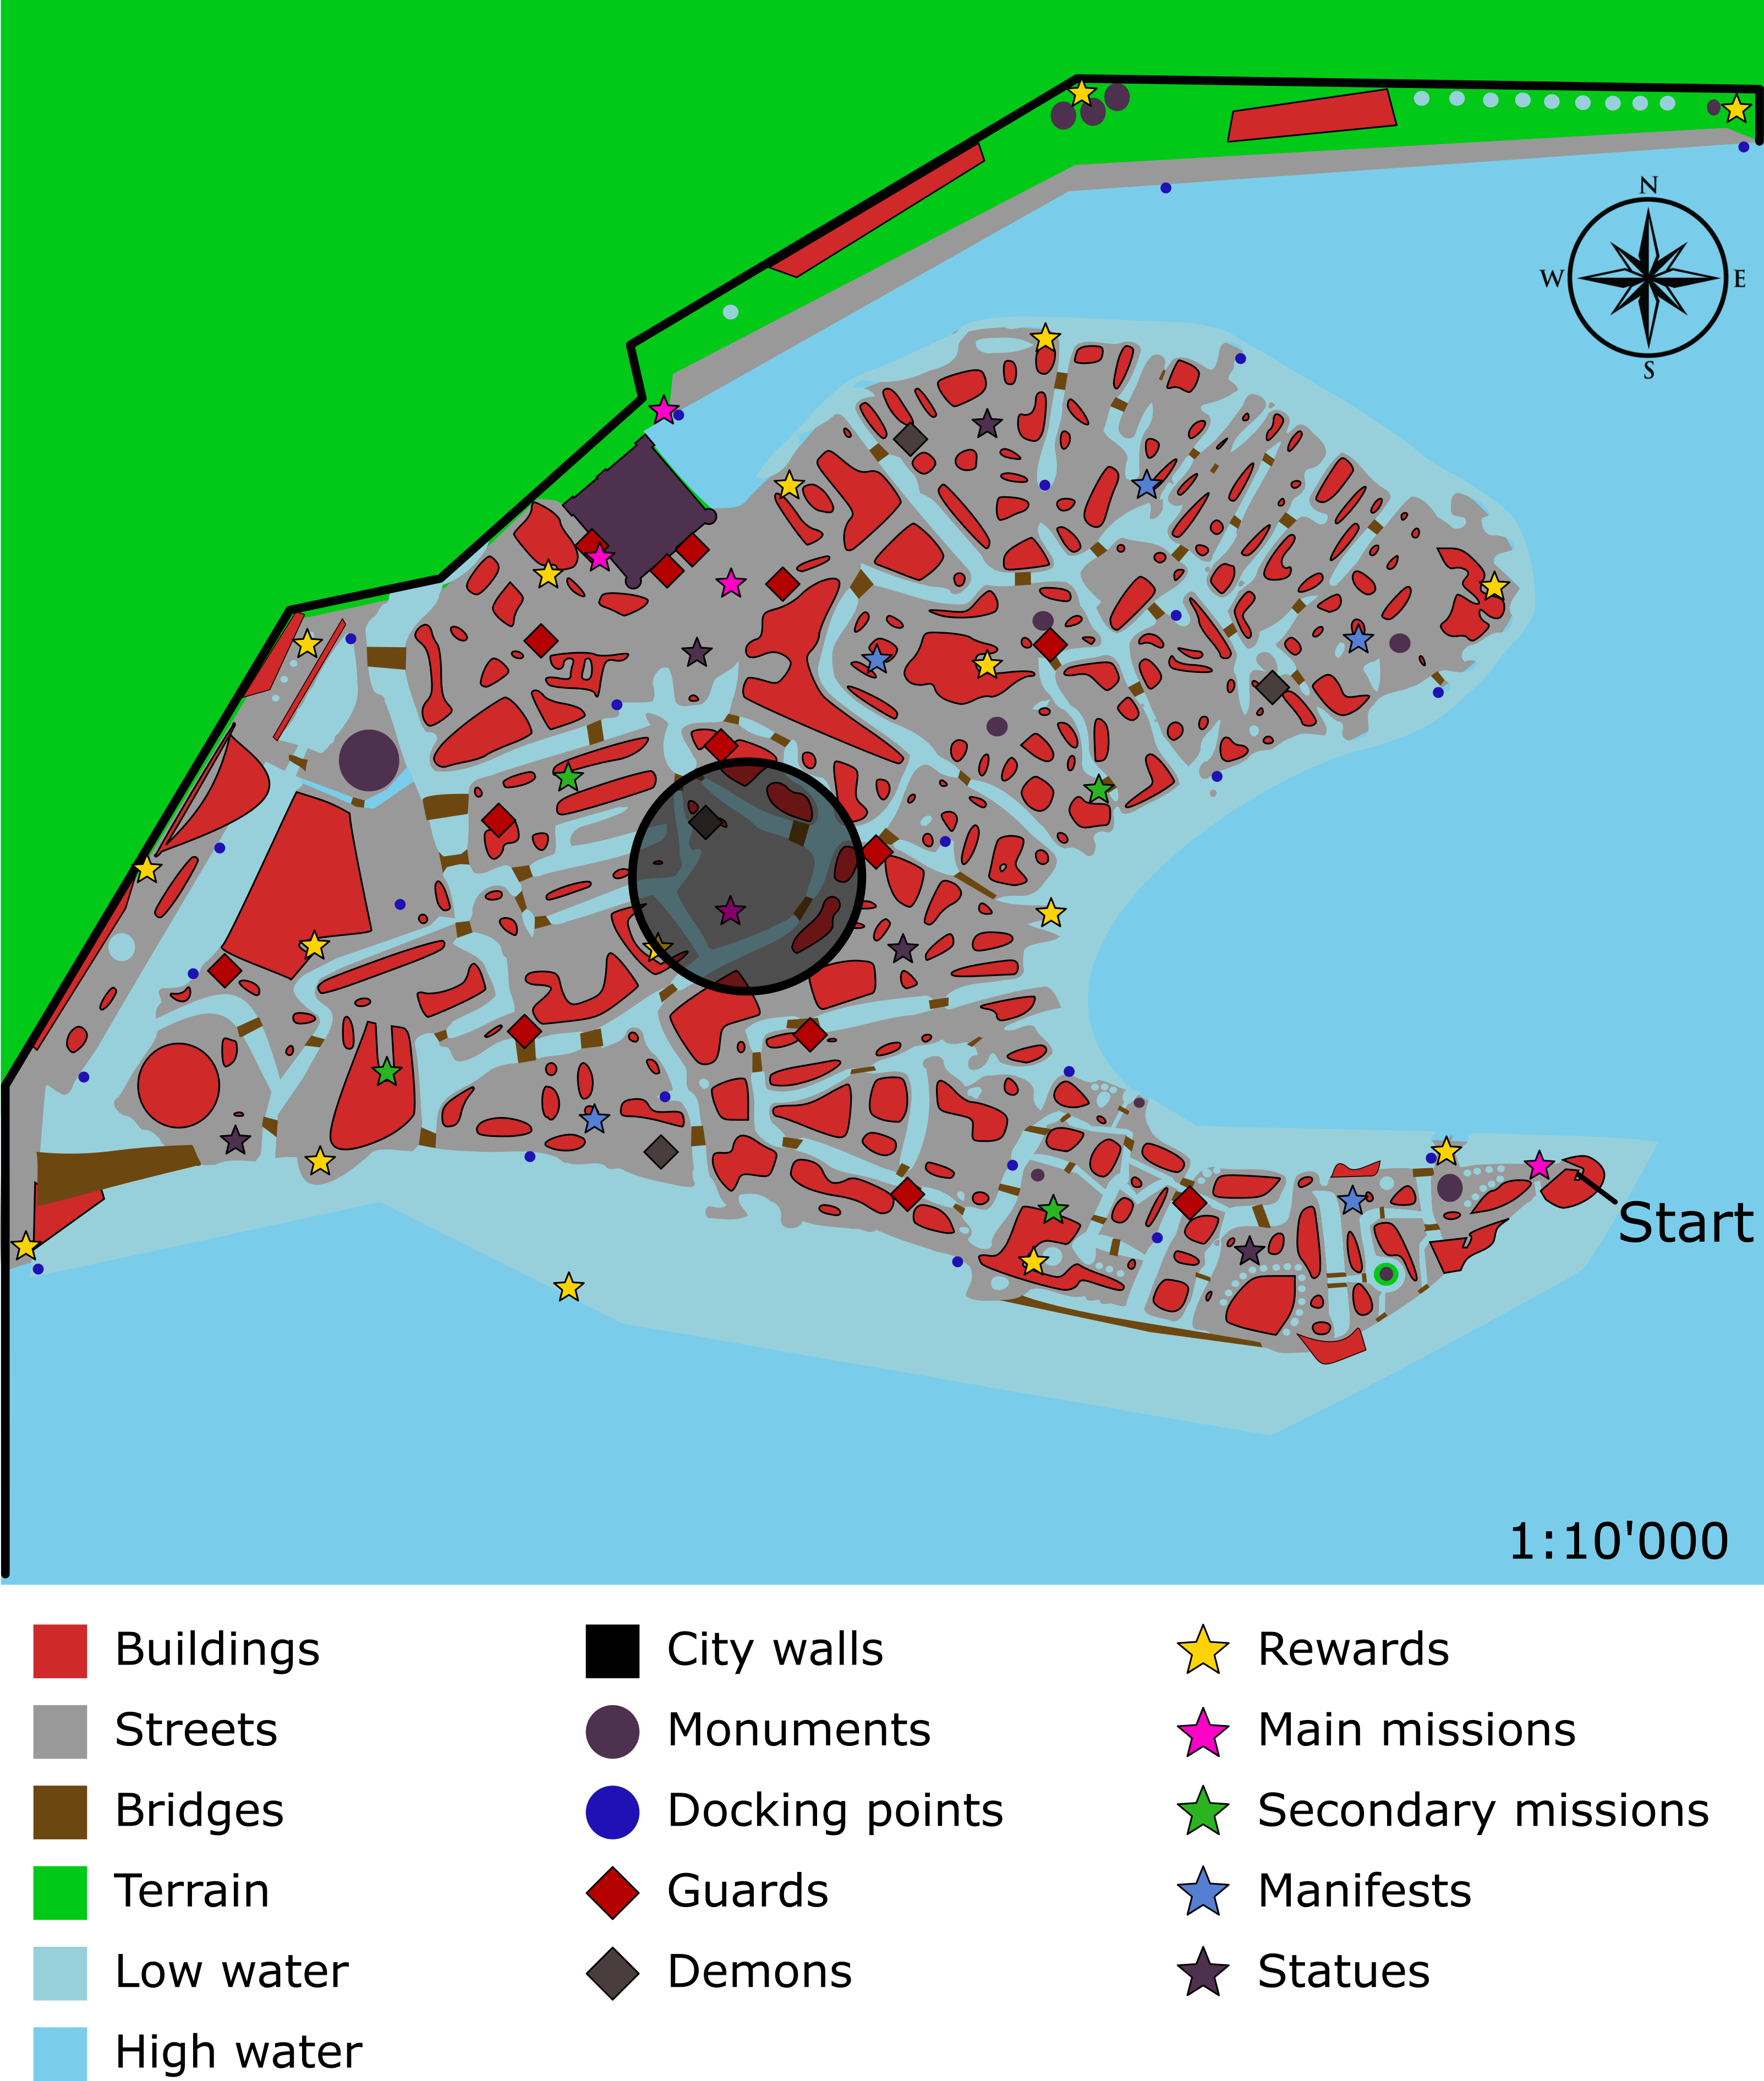
\includegraphics[width=12cm]{Images/Maps/dynamia_market}
  \caption{Market position}
\end{figure}

The Market is situated in a wide square positioned in the middle of the city. It is surrounded by many canals and it is the nerve centre of Dynamia where, everyday, people and merchants from every part of the region come to buy and sell any kind of merch. There are many stands that sell clothes, hats, wool and fabric and here the player could find some of the rarest materials to craft items. \\
The market is characterized by a constant buzz caused by the huge crowd that populates  the square during the daytime. During the late afternoon merchants and people start leaving the market and so it becomes a quiet place where Dynamians love to stay and walk in the evening.
In the south west corner the player will find the merchant that will help in finding a way to get inside the castle.
 
\begin{figure}[H]
  \centering
  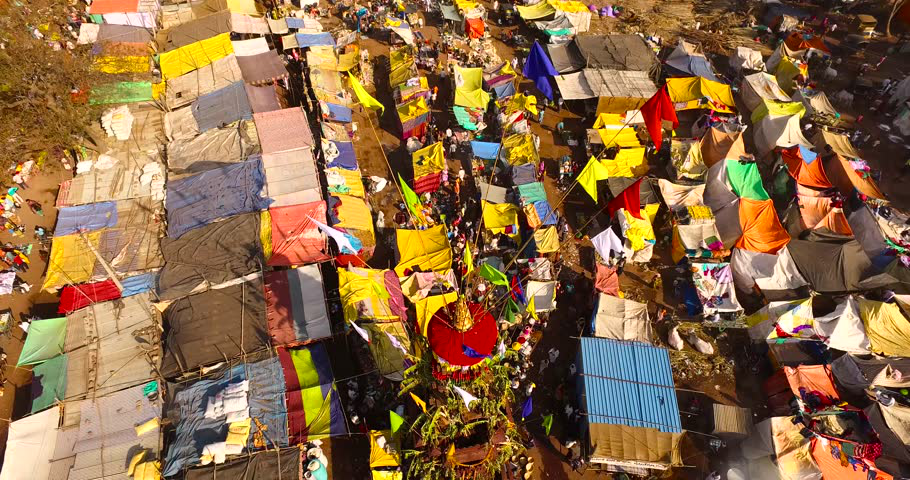
\includegraphics[width=\textwidth]{Images/Landmarks/market}

  \caption{Reference image for the market}
    For more reference images: \href{http://wastelandsteam.altervista.org/dynamia-dead-end}{http://wastelandsteam.altervista.org/dynamia-market}\\Password: \textit{gld18}
\end{figure}

\subsection{Castle of Dynamia}
\begin{figure}[H]
  \centering
  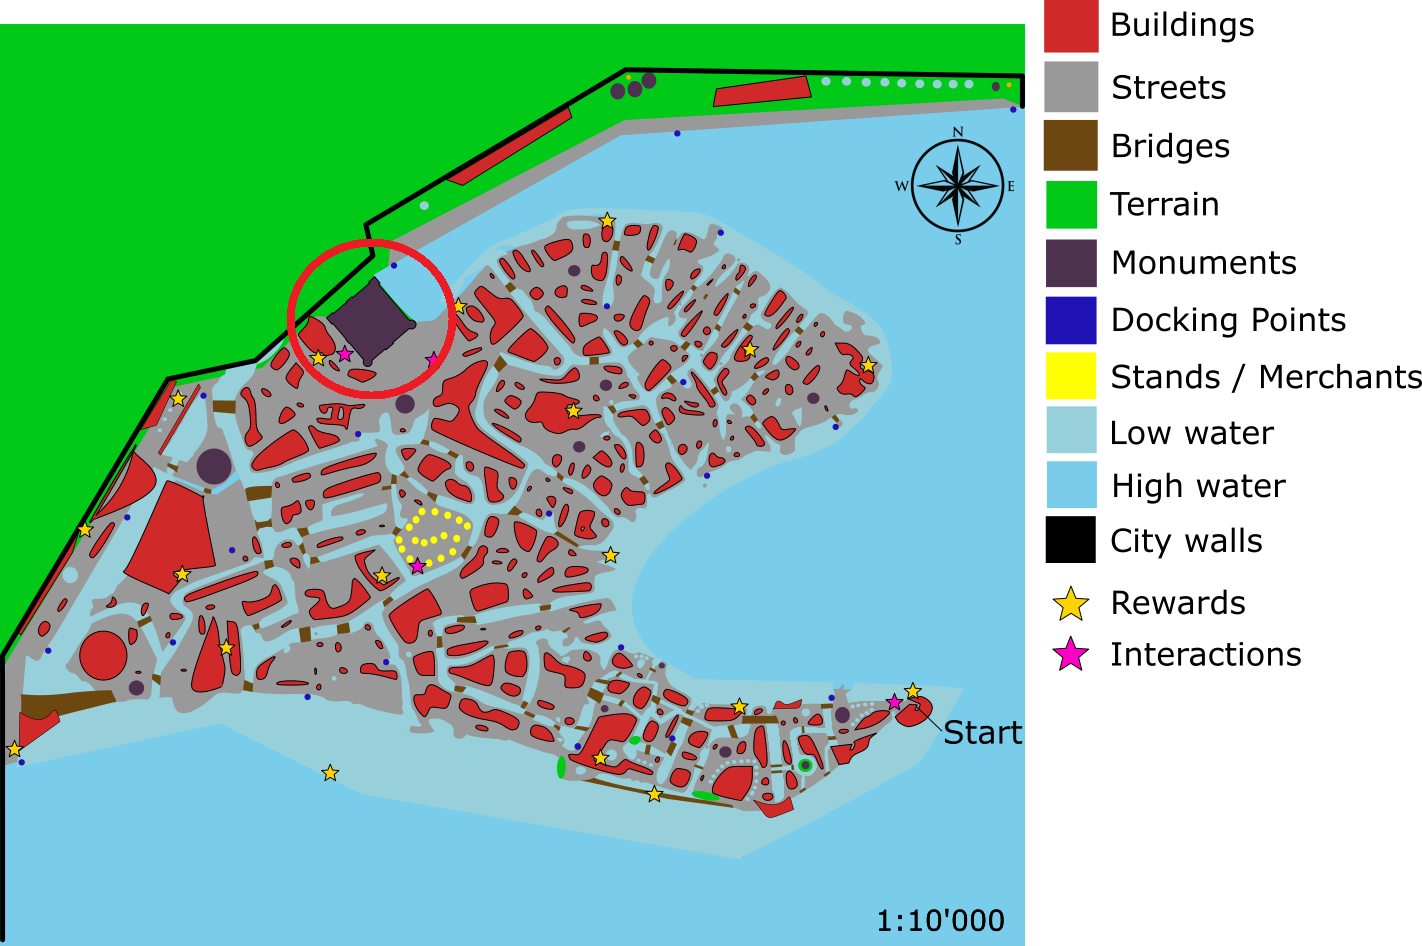
\includegraphics[width=12cm]{Images/Maps/dynamia_castleOfDynamia}
  \caption{Castle position}
\end{figure}

The castle of Dynamia is loosely based on the Sforza Castle of Milan.

\begin{figure}[H]
  \centering
  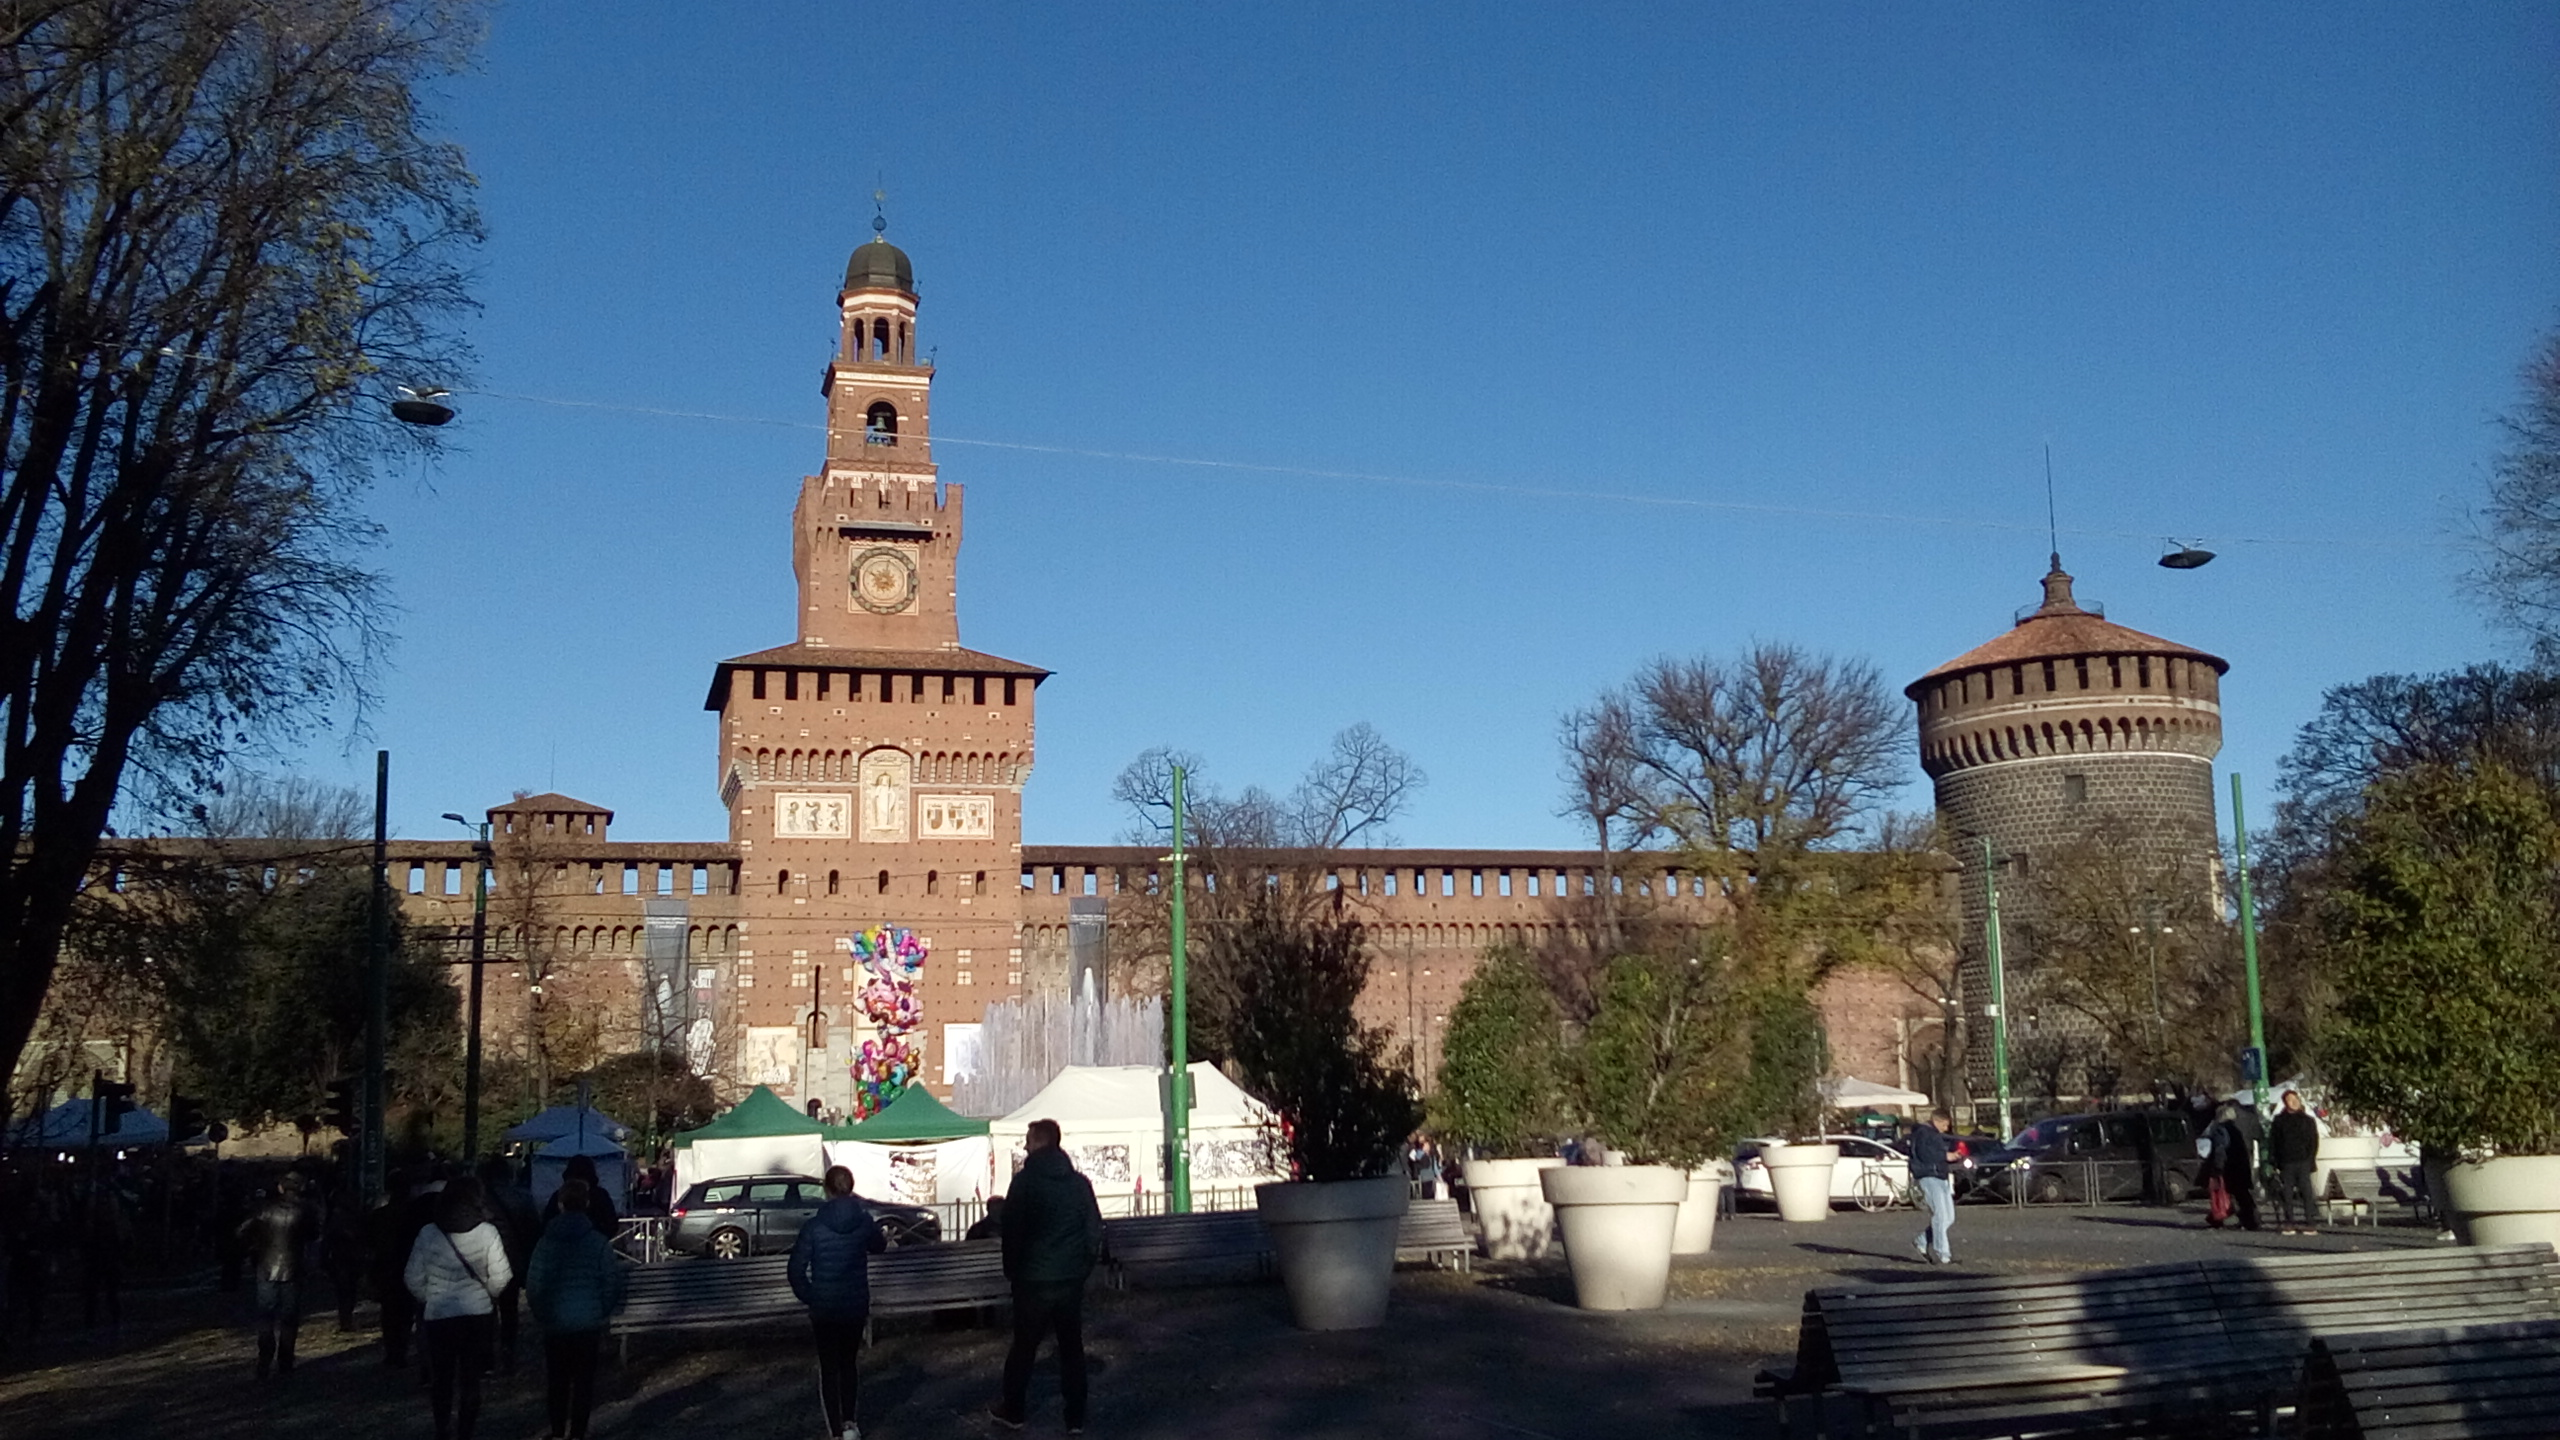
\includegraphics[width=\textwidth]{../../../References/Images/Dynamia/CastleOfDynamia/20181208_100357}
  \caption{Reference image for the Castle of Dynamia}
\end{figure}

It is placed upon a rocky promontory and it is the main entrance to Dynamia from the continent. It has been designed by the court magician of Dynamia centuries ago, and it has many secret passages. The player can access some of this secret passages by solving puzzles.

It is made of stones, it has a big courtyard and two buildings: one on the west, heavily fortified, and one, more refined, on the north for the royal family. Mizar lives in the northern building, but the player can visit only the courtyard and the western area.

There are human guards and demons that patrol the castle. They are ordered to arrest any intruder. The most powerful enemy is the captain of the guards.

\begin{figure}[H]
  \centering
  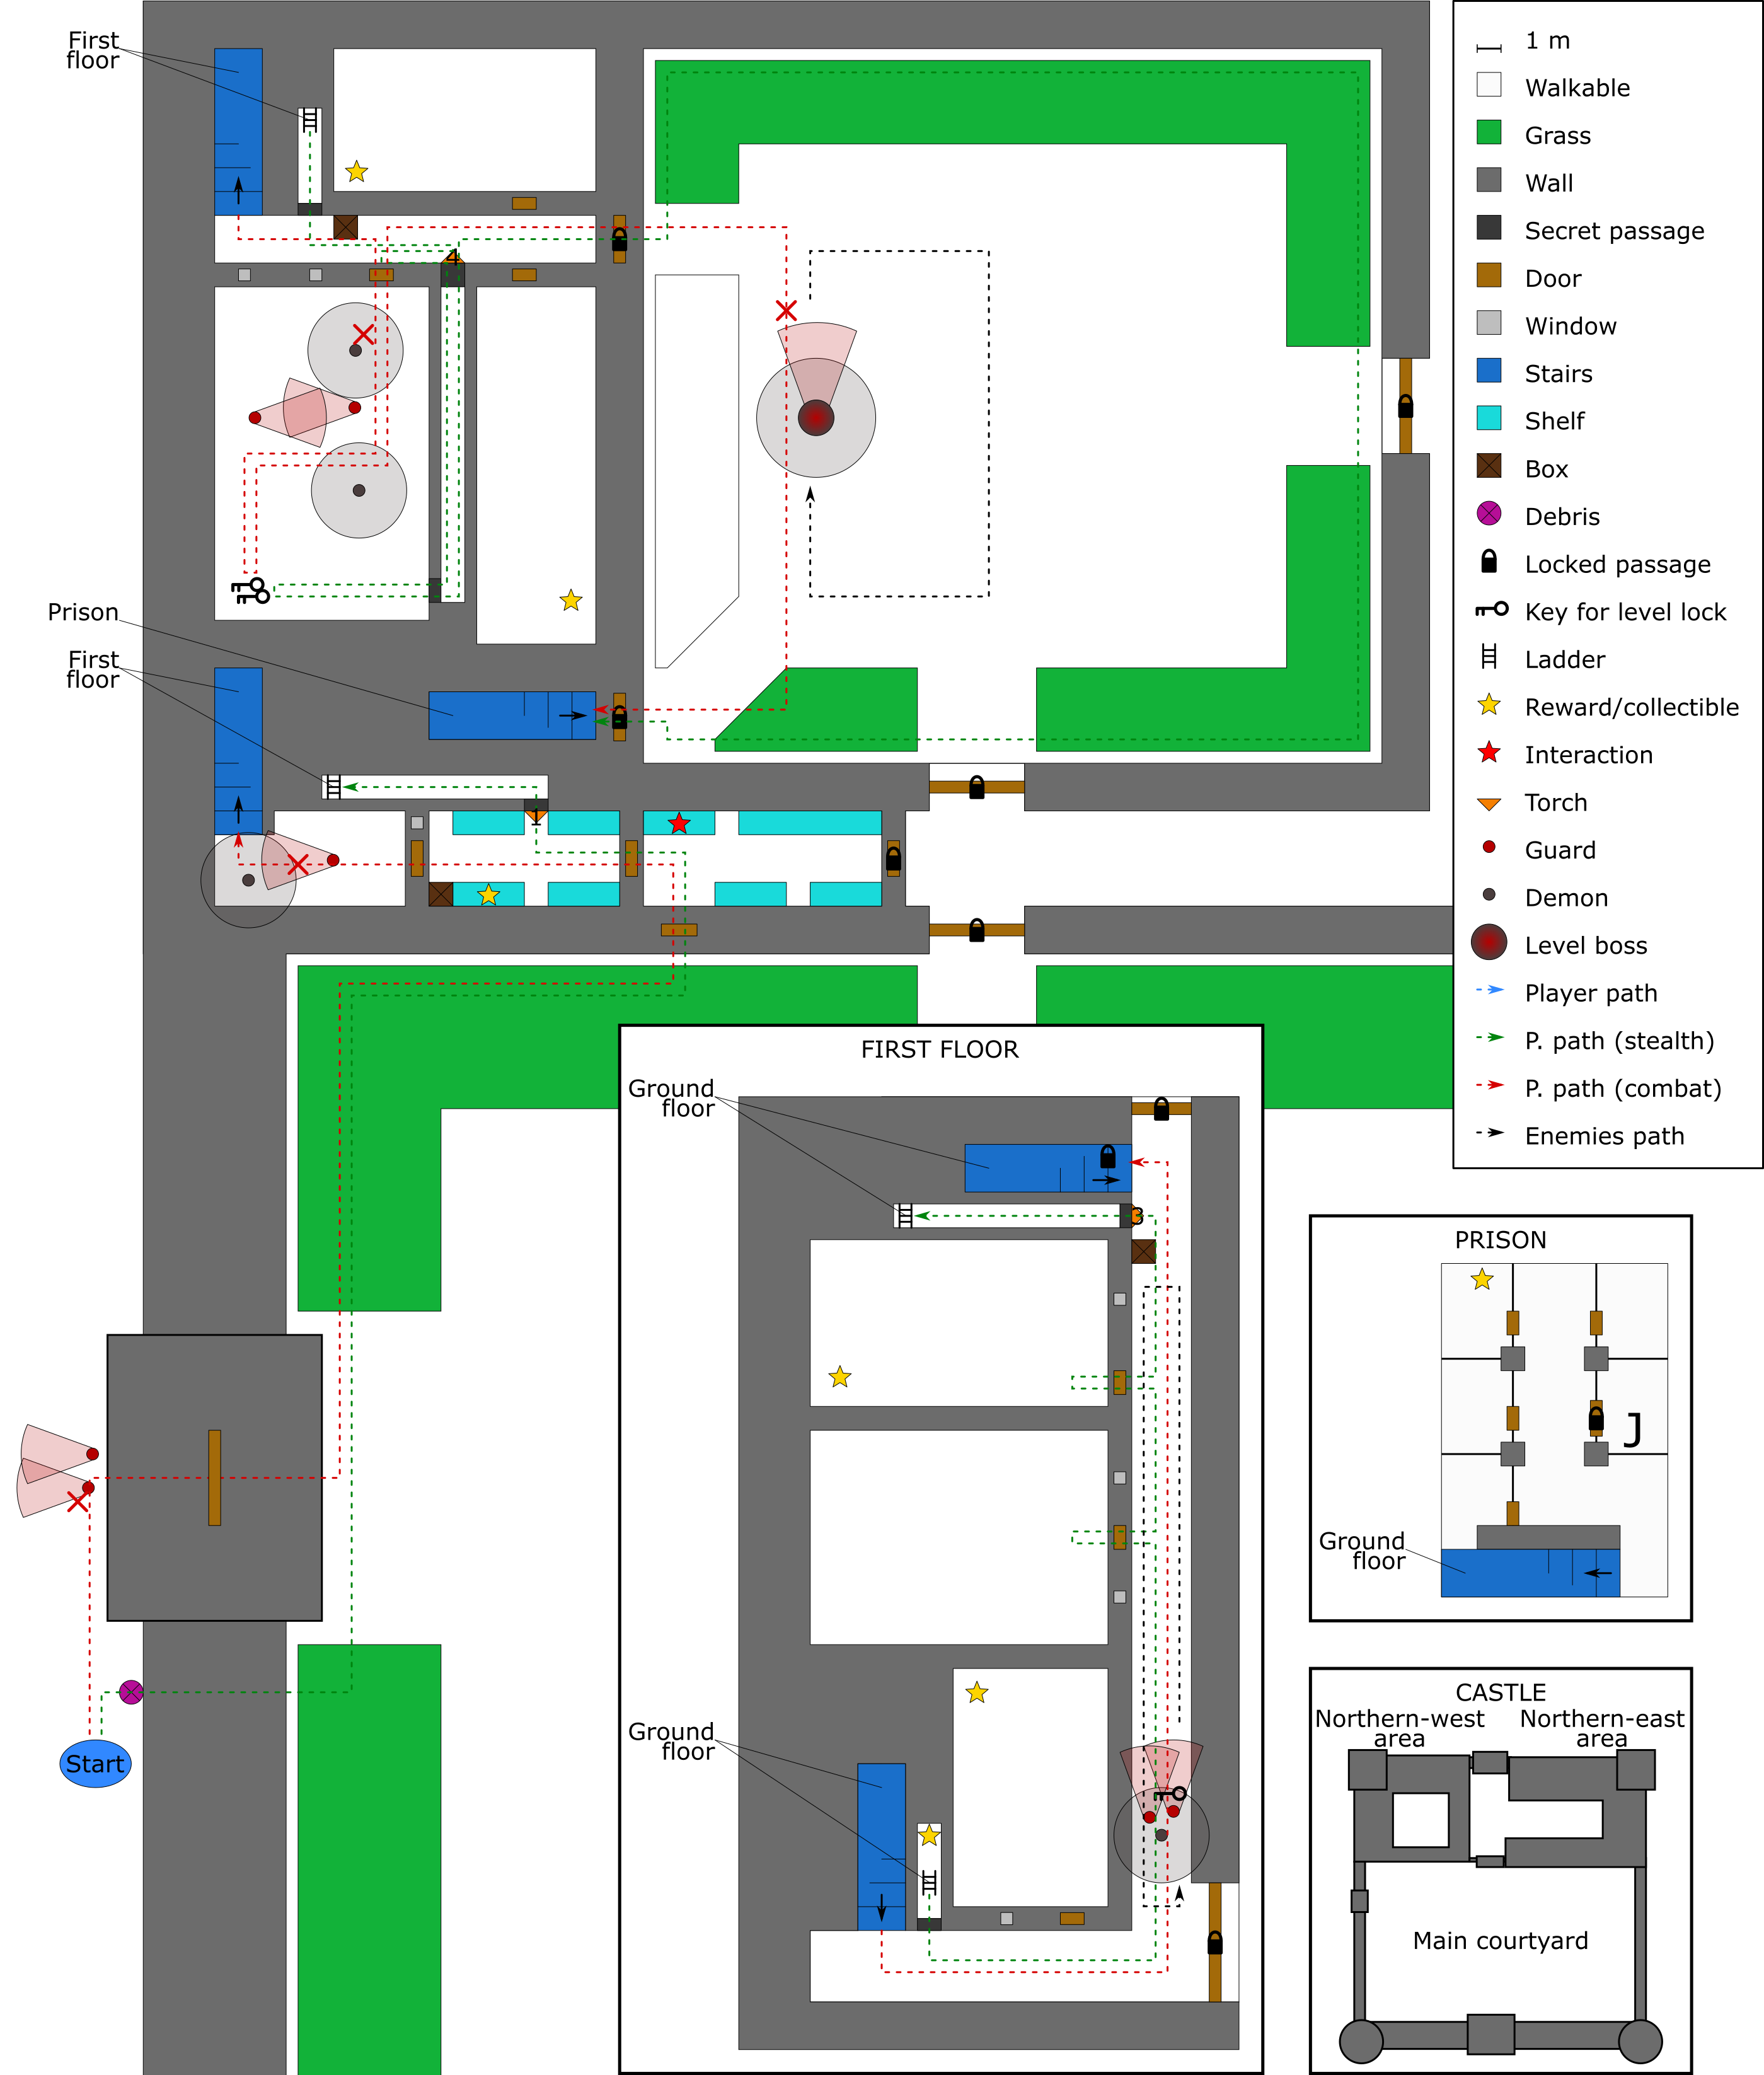
\includegraphics[width=\textwidth]{Images/Maps/castleOfDynamia}
  \caption{Map of the Castle of Dynamia}
\end{figure}

\subsubsection{Puzzles}
While exploring the castle, the player can choose to solve some puzzles and, by so, avoid fighting some enemies.

\subsubsection*{1. Build a machine}

\begin{figure}[H]
  \centering
  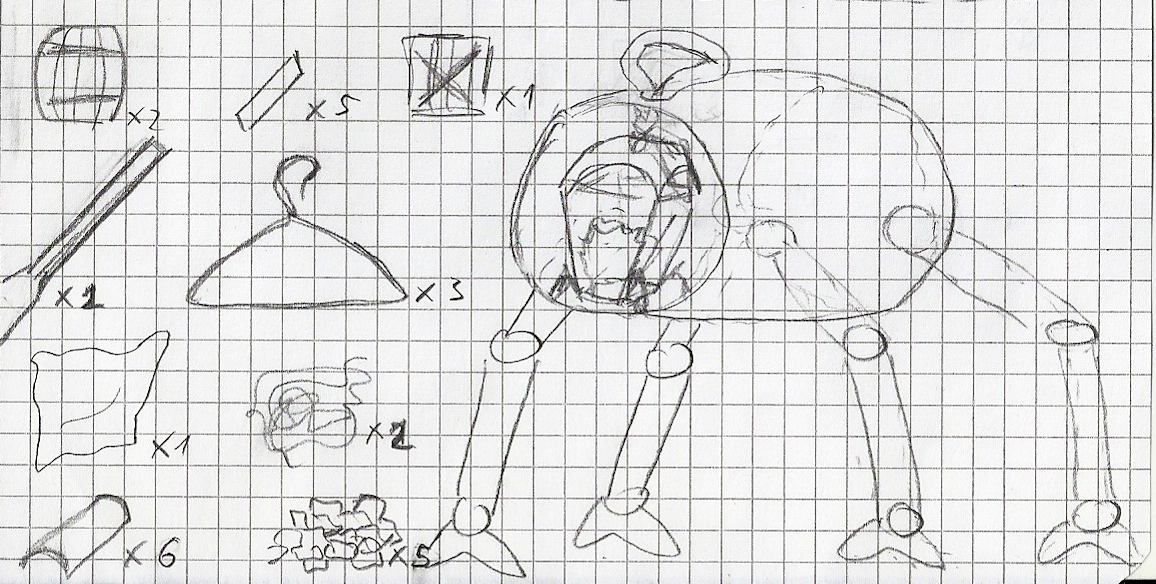
\includegraphics[width=\textwidth]{Images/Puzzles/castleOfDynamia_1}
  \caption{Puzzle 1 in the Castle of Dynamia}
\end{figure}

In order to enter in the courtyard the player can use some debris to build a machine for Calcifer that allows him to climb the wall without being detected.

The player has different parts and he/she has to understand how to combine them. He/She has to break some part to obtain new components. Some parts are not required to build the machine.

\subsubsection*{2. Rotate the torch}

\begin{figure}[H]
  \centering
  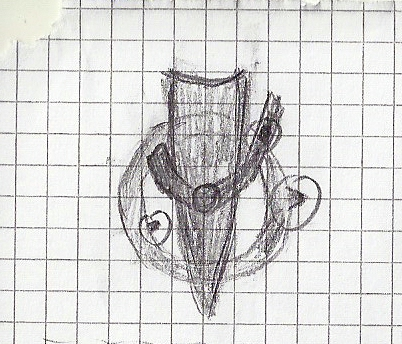
\includegraphics[width=\textwidth]{Images/Puzzles/castleOfDynamia_2}
  \caption{Puzzle 2 in the Castle of Dynamia}
\end{figure}

The torch is a puzzle itself. The player has to rotate the torch and its arms according to the given scheme.

When the player rotates the main body, the two arms rotate too. When he/she rotates an arm, the main body rotates too, but the other arm stays still.

\subsubsection*{3. Press the bricks}

\begin{figure}[H]
  \centering
  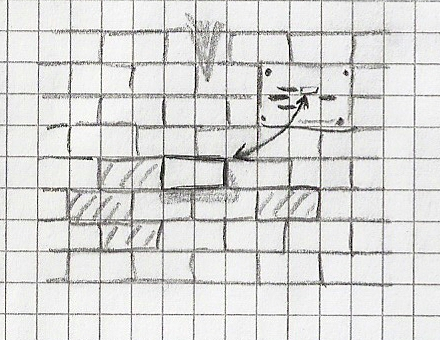
\includegraphics[width=\textwidth]{Images/Puzzles/castleOfDynamia_3}
  \caption{Puzzle 3 in the Castle of Dynamia}
\end{figure}

Near the torch there is a small plate with some horizontal lines. The player has to press the bricks in the corresponding position under the torch.

A protruding brick helps the player to identify the bricks to press.

\subsubsection*{4. Connect the cables}

\begin{figure}[H]
  \centering
  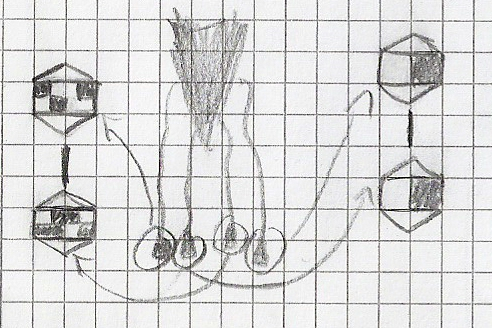
\includegraphics[width=\textwidth]{Images/Puzzles/castleOfDynamia_4}
  \caption{Puzzle 4 in the Castle of Dynamia}
\end{figure}

There are some cables that hang under the torch. The player has to connect them in the correct pairs, according to the pattern on the plugs.

\subsection{Docking point}
\begin{figure}[H]
  \centering
  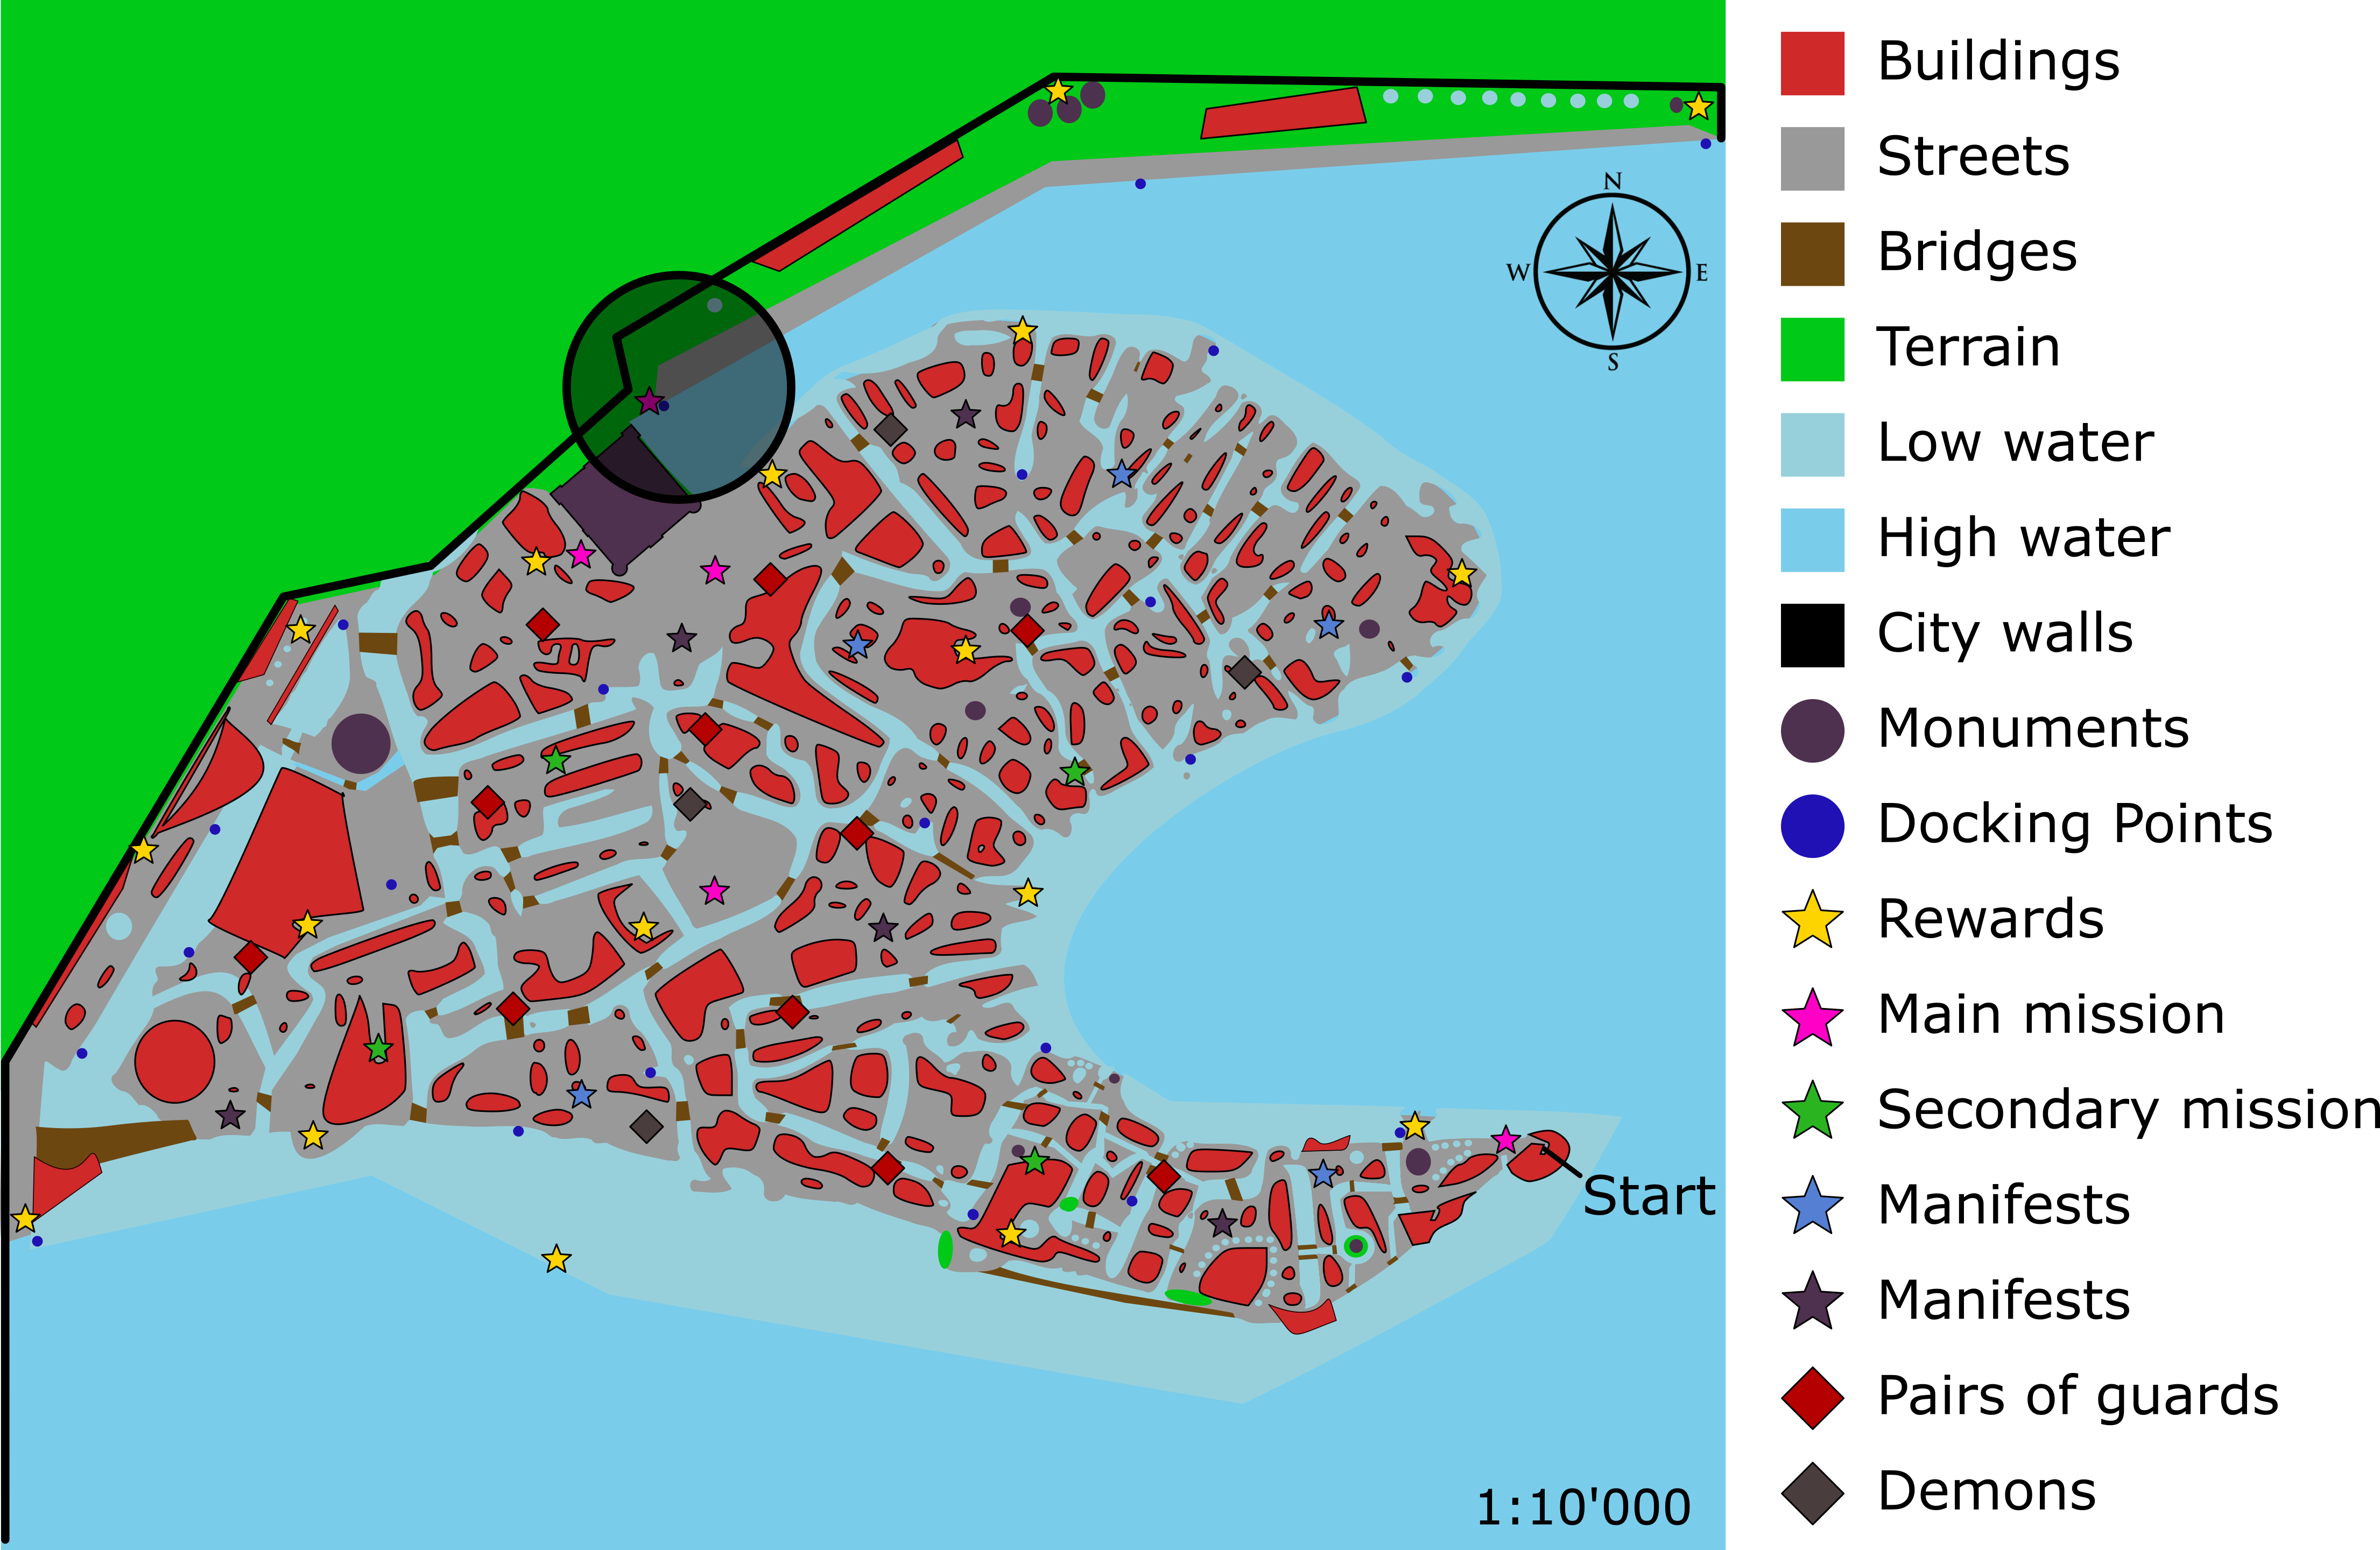
\includegraphics[width=12cm]{Images/Maps/dynamia_dockingPoint}
  \caption{Docking point position}
\end{figure}
  
In this area we may find wooden poles placed in the water, decorated with flowers, where gondoliers and fishers tie their little boats and gondolas, and  stone stairs that lead to small platforms on the canals. 
In the center of the area there is a small street and a fountain which has in its middle a statue representing Mizar, surrounded by flowers. Mizar keeps her right arm up holding her scepter that spills water.
Behind the docking point the player can see the gigantic city walls that defend Dynamia from enemy attacks.
\begin{figure}[H]
    \centering
    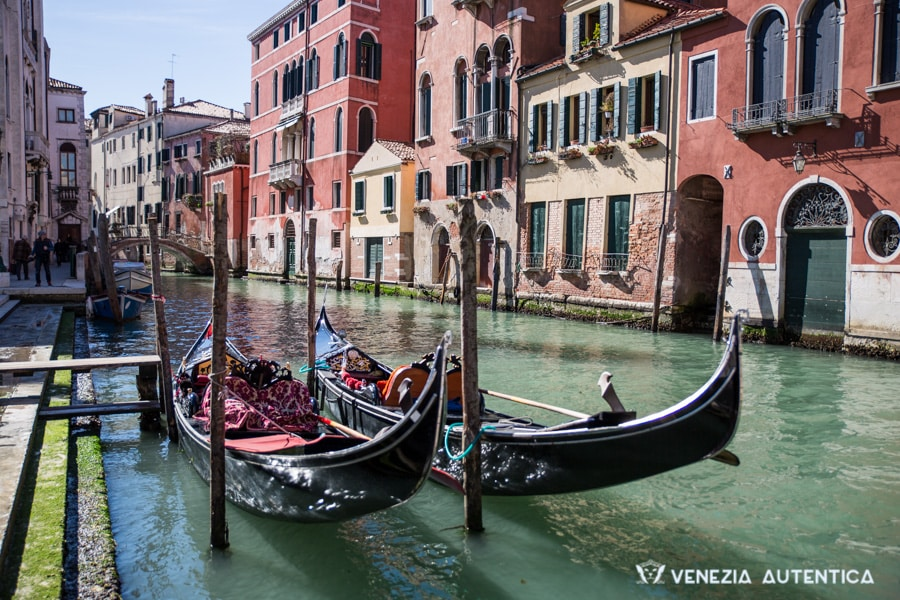
\includegraphics[width=8cm]{Images/Landmarks/dockingPoint}
    \caption{References image for the docking point}
    For more reference images: \href{http://wastelandsteam.altervista.org/dynamia-docking-point}{http://wastelandsteam.altervista.org/dynamia-docking-point}\\Password: \textit{gld18}
  \end{figure}
